\chapter{2D Simulations - OFETs}
\label{sec:ofet}

\begin{figure}[H]

\begin{tabular}{ c l }


\includegraphics[width=0.05\textwidth]{./images/youtube.png}

&
\href{https://www.youtube.com/watch?v=0RK9GEyb4HQ}{Tutorial on OFET simulation.}

\end{tabular}
\end{figure}

OghmaNano contains a 2D electrical solver that can be used for simulating OFETs and other 2D structures.  To perform 2D simulations use the default OFET simulation in OghmaNano as a starting point.  You can do this by double clicking on \emph{OFET simulation} in the new simulation window (see figure \ref{fig:ofetnewsim}).
\\
\\
\fbox{
\parbox{0.9\textwidth}{
\color{black} Note: The 2D electrical solver is a separate plug in to the 1D solver, if you select the default OFET simulation OghmaNano as a starting point for your own 2D simulations OghmaNano will be all set up to do 2D electrical simulations.  If you try to convert a 1D simulation such as a solar cell to a 2D simulation (not recommended) please read section \ref{sec:solverconfig} on how to select the correct solver.
}\par
}
\\
\\
\\
To make a new OFET simulation, click on the new simulation button. In the new simulation window and select the OFET simulations (see figure \ref{fig:ofetnewsim0}).  Double clicking on this will bring up the OFET sub menu, where other types of OFETs are also stored. There is one example with a top contacts, one with side contacts and one which is at low temperature. For this capter we will be looking at the (standard) top contact OFET (Figure \ref{fig:ofetstartsim1}), double click on this and save the new simulation to disk.
\\
\\
\noindent
\begin{minipage}{0.5\textwidth}
	\centering
	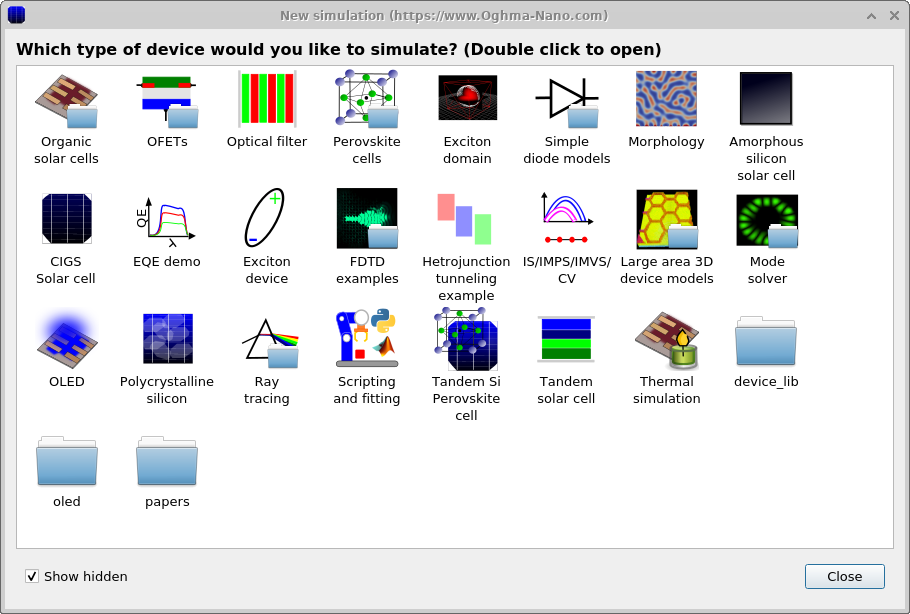
\includegraphics[width=\linewidth,height=0.8\linewidth]{./images/ofet/ofet_new_sim0.png}
	\captionof{figure}{Setlect the OFET submenu to main a new OFET simulation}
	\label{fig:ofetnewsim0}
\end{minipage}
\hspace{4pt}
\begin{minipage}[]{0.5\linewidth}
	\centering
	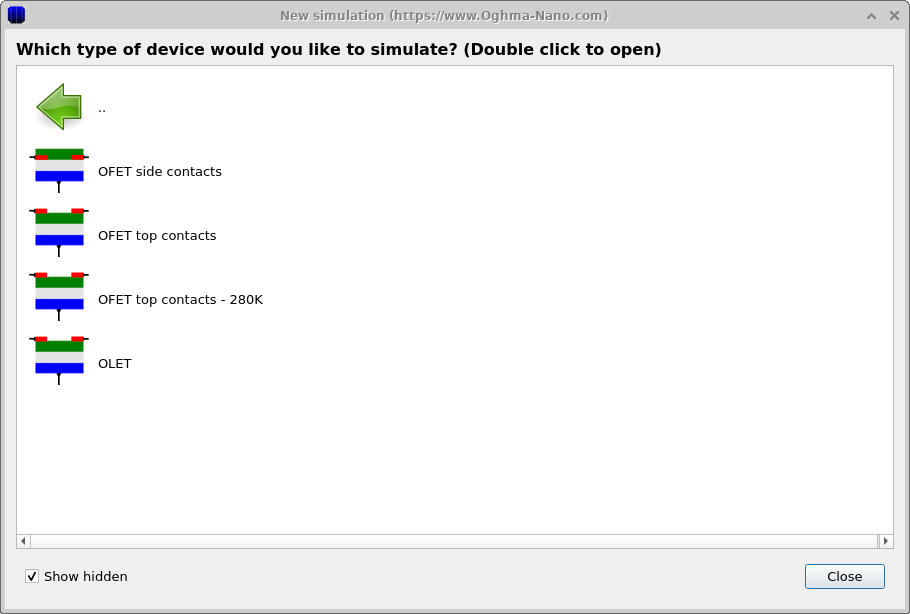
\includegraphics[width=\linewidth,height=0.8\linewidth]{./images/ofet/ofet_new_sim1.png}
	\captionof{figure}{Select the OFET top contact for this example.}
	\label{fig:ofetnewsim1}
\end{minipage}


\subsection{The anatomy of a 2D simulation}

\begin{figure}[H]
\centering
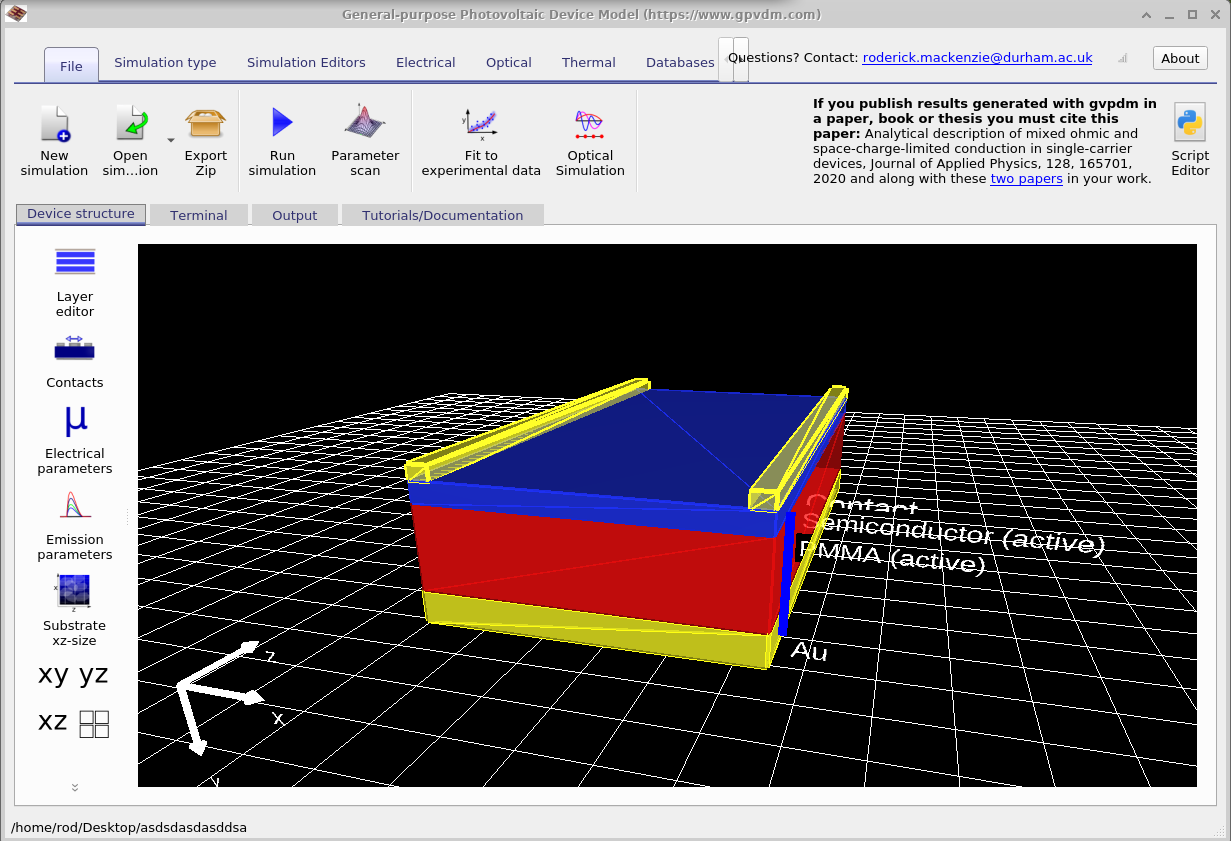
\includegraphics[width=0.7\textwidth]{./images/ofet/ofet_1.png}
\caption{The default ofet simulation.}
\label{fig:ofetstartsim}
\end{figure}

The OFET structure shown in Figure \ref{fig:ofetstartsim} has three contacts, a \emph{gate}, \emph{source} and a \emph{drain}. The source and drain are shown on the top of the simulation as gold bars, a semiconductor layer is shown in blue and an insulating later shown in red.  The \emph{gate} contact is visible at the bottom of the structure.  This layered structure is defined in layer editor, see figure \ref{fig:ofetlayerstructure}. The layer editor has been described in detail in section \ref{sec:layereditor}. It can be seen that the top and bottom layers have been set to \emph{contact} and the insulator (PMMA) and semiconducting layer have been set to active. This means that the electrical model will only consider the semiconductor and insulator layers and the contacts will be used as boundary conditions.  As this structure is not emitting light the \emph{Optical material} column has no impact on the simulation results so it has been arbitrary materials.

\begin{figure}[H]
\centering
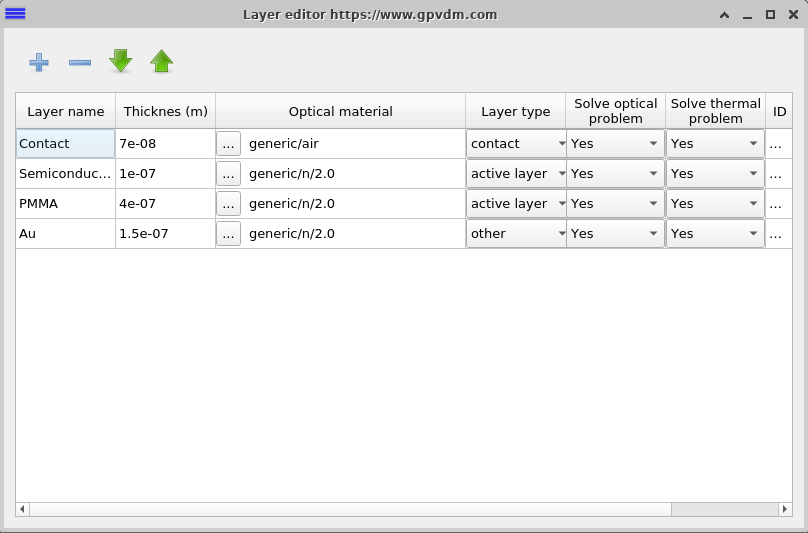
\includegraphics[width=0.7\textwidth]{./images/ofet/ofet_2.png}
\caption{The layers of an OFET device}
\label{fig:ofetlayerstructure}
\end{figure}

The contacts are defined in the contact editor shown in Figure \ref{fig:ofetcontacteditor}. The contact editor has been described in detail in 
section \ref{sec:contacteditor}, however because this is a 2D simulation another two extra columns have appeared. They are \emph{start} and \emph{width}.  These define the start position of the contact on the x-axis and width which describes the width of the contact on the x-axis.  The \emph{source} starts at $0~m$ and extends to $5 \mu m$, the  \emph{drain} starts at $75~\mu m$ and extends to $5 \mu m$, while the gate starts at $0~m$ and extends to cover the entire width of the device which is $80~ \mu m$.  If you are unsure which is the x-axis, the origin marker is visible at the bottom of figure \ref{fig:ofetstartsim}. Notice also that under the column \emph{Applied Voltage}, the \emph{source} is marked \emph{Ground} this means that 0V will be applied to the ground, the \emph{gate} is marked \emph{change} meaning that our voltage ramp as defined in the JV editor will be applied to this contact, and the \emph{drain} is marked \emph{constant bias} with a voltage of 15V, this means that a constant voltage of 15V will be applied to this contact. And thus we are scanning the gate contact while applying a constant voltage between the source and the drain.

\begin{figure}[H]
\centering
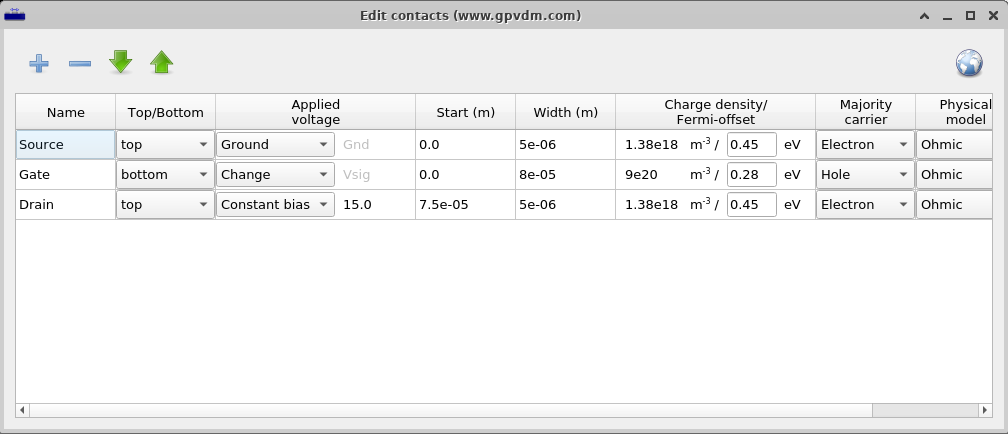
\includegraphics[width=0.7\textwidth]{./images/ofet/ofet_3.png}
\caption{Editing the contacts on a 2D device.}
\label{fig:ofetcontacteditor}
\end{figure}

\subsection{Electrical parameters}
\subsubsection{Disabling drift diffusion in the insulator layer}
The electrical parameters for both the semiconductor and the insulator can be seen in Figure \ref{fig:ofetelectricalparamters}, these can be accessed through the \emph{Electrical parameter} editor. The \emph{Electrical parameter} editor is described in detail in section \ref{sec:doseditor}. The left image shows the parameters for the semiconducting layer while the right figure shows the parameters for PMMA. If you look in the top left of both windows you will see a button called \emph{Enable Drift Diff.} which stands for \emph{Enable Drift Diffusion}. When this is depressed the drift diffusion equations will be solved within the layer which take into account charge movement. When this is not depressed only Poisson's equation will be solved in the layer and the movement of charge ignored. If you notice this button is depressed in the Semiconductor layer and not depressed in the PMMA insulator.  This means that the drift-diffusion equations will be solved in the semiconductor and not in the PMMA. The reason for doing this is that charge does not conduct in the PMMA so there is no point in solving the drift-diffusion equations in that layer. Another approach would be to solve the drift-diffusion equations in both layers and just set the mobility in the PMMA to be very low but this will result in slower computational times and is less numerically stable, there is more on this approach below.

\begin{figure}[H]
\centering
\begin{tabular}{ c c }

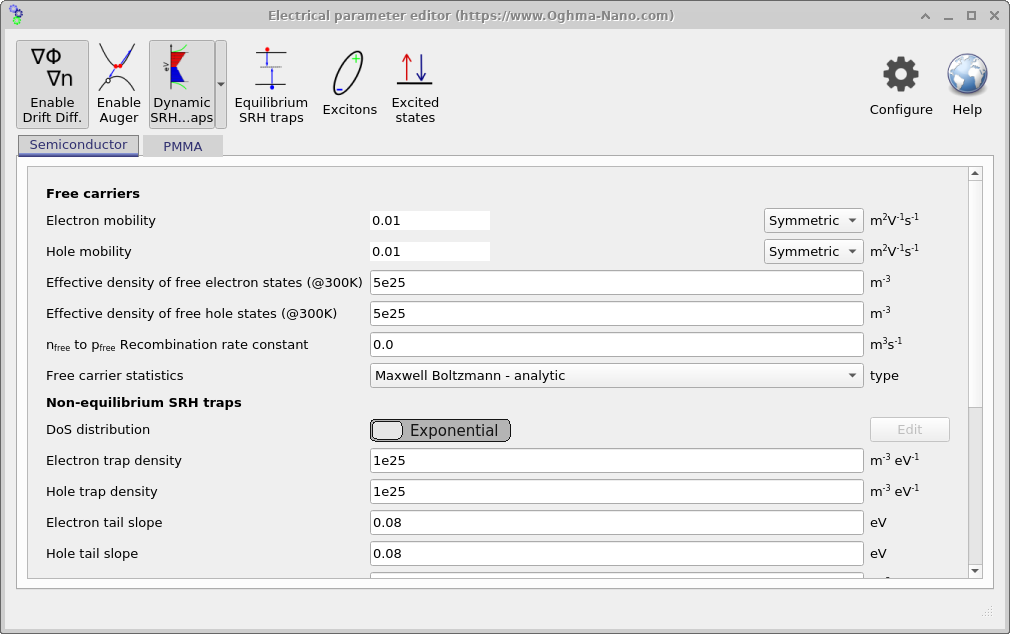
\includegraphics[width=0.5\textwidth,height=0.35\textwidth]{./images/ofet/ofet_5.png}

&
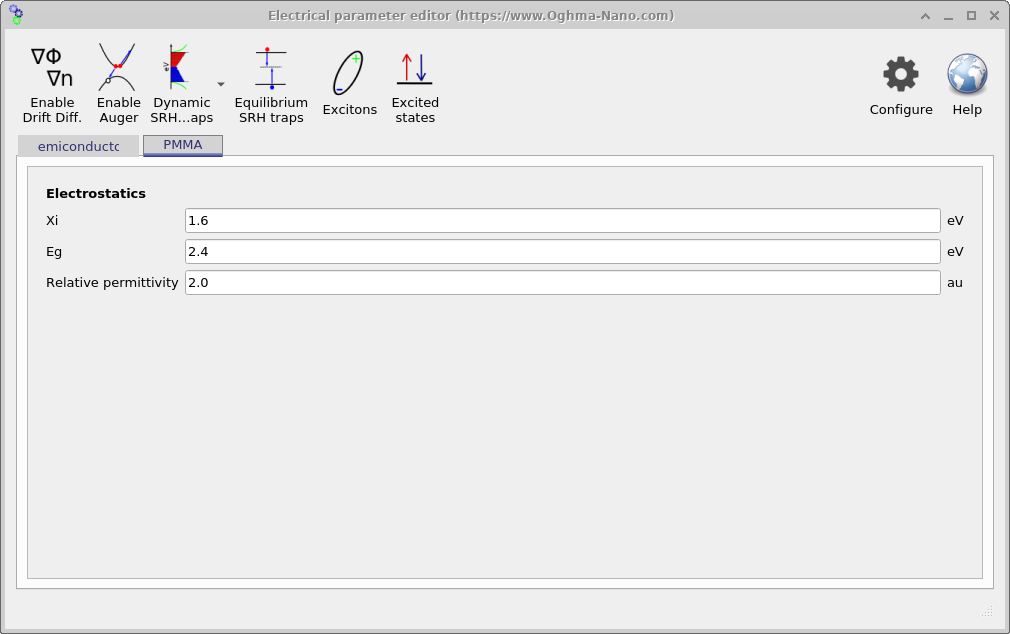
\includegraphics[width=0.5\textwidth,height=0.35\textwidth]{./images/ofet/ofet_6.png}
\\
\end{tabular}
\caption{Electrical parameters for both the semiconductor (left) and the insulator (right)}
\label{fig:ofetelectricalparamters}
\end{figure}

\subsection{Running a 2D simulation}

2D simulations are run in the same way as 1D simulations, simply click on the play button, see figure \ref{fig:ofetrun}.
\begin{figure}[H]
\centering
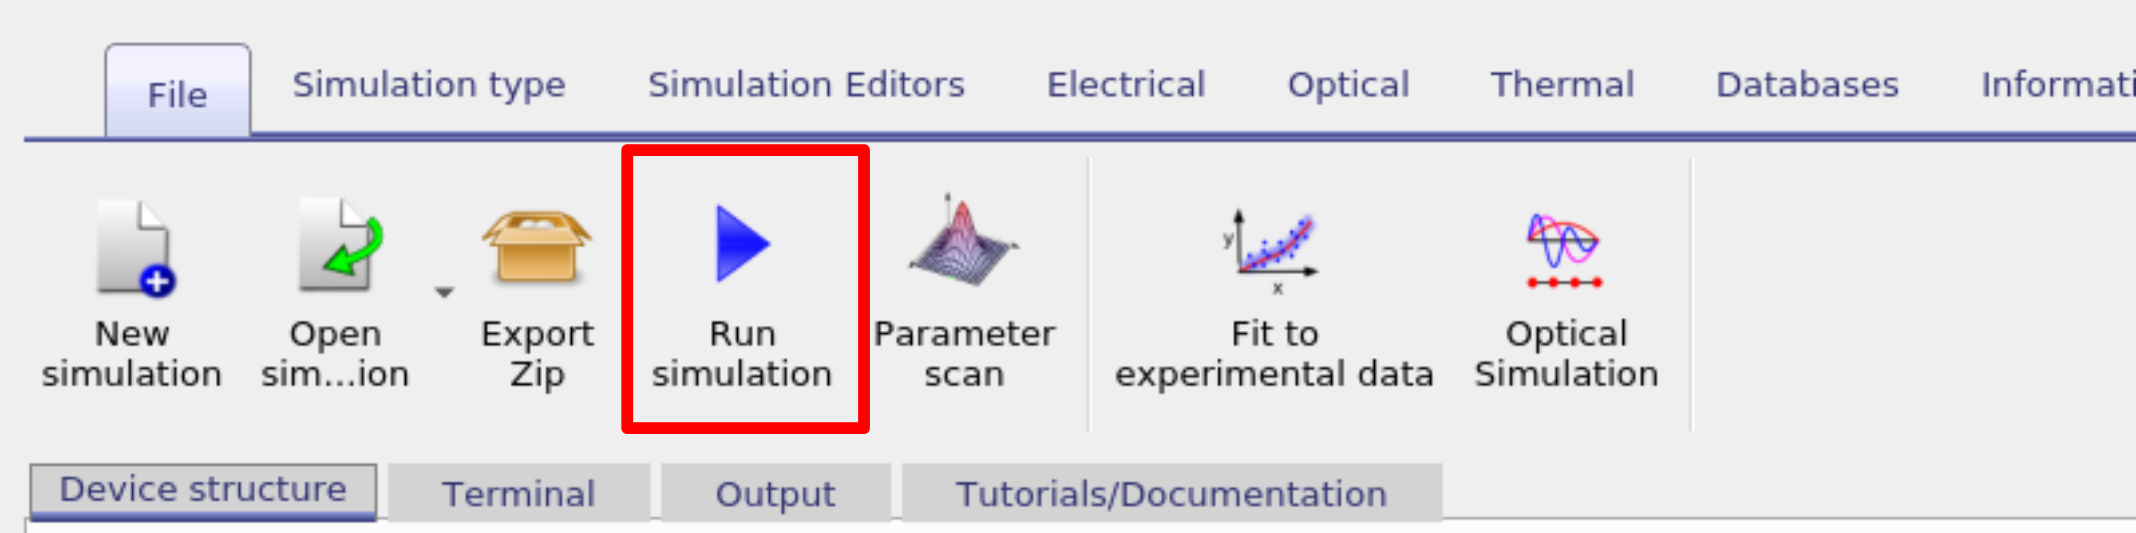
\includegraphics[width=0.7\textwidth]{./images/run_sim.png}
\caption{Running an OFET simulation}
\label{fig:ofetrun}
\end{figure}

The simulation will take longer than it's 1D counterparts simply because there will be more equations to solve.  If you have set a contact at a high starting voltage the solver will initially ramp the contact voltage in a stepwise way until the desired voltage is achieved before the desired voltage sweep is applied to the \emph{active contact}. After the simulation has run the following files will be produced showing the current density from each contact.

\begin{table}[H]
\begin{center}
\begin{tabular}{ |c|c| } 
 \hline
	File name 			& 	Description  \\ 
 \hline
	$contact\_iv0.dat$	&	Current voltage current curve for contact 0 \\ 
	$contact\_iv1.dat$	&	Current voltage current curve for contact 1 \\ 
	$contact\_iv2.dat$	&	Current voltage current curve for contact 2 \\ 
	$contact\_jv0.dat$	&	Current density voltage current curve for contact 0 \\
	$contact\_jv1.dat$	&	Current density voltage current curve for contact 1 \\
	$contact\_jv2.dat$	&	Current density voltage current curve for contact 2 \\
	snapshots	&	Simulation snapshots \\
 \hline
\end{tabular}
\caption{Files produced by the steady state OFET simulation}
\label{tab:ofet_jv_output}
\end{center}
\end{table}

Contacts in OghmaNano are labelled from 0 to N in the order they are defined in the contact editor (see Figure \ref{fig:ofetcontacteditor}), so in this case Contact 0 will be the source, contact 1 will be the gate and contact 2 will be the drain. You can see the result of running the simulation in Figure \ref{tab:ofet_plots}.
\begin{figure}[H]
\centering
\begin{tabular}{ c c }

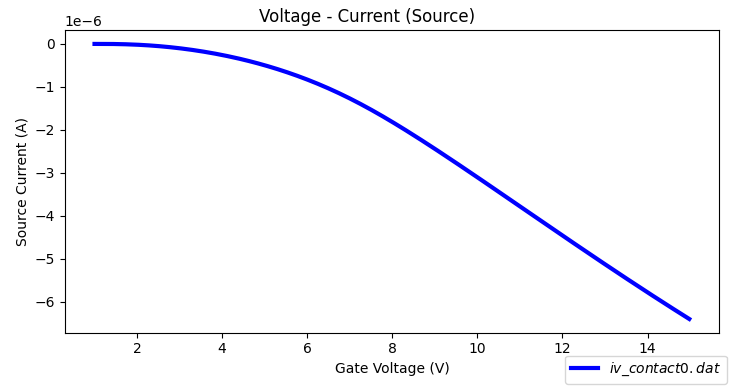
\includegraphics[width=0.5\textwidth,height=0.4\textwidth]{./images/ofet/ofet_7.png}

&
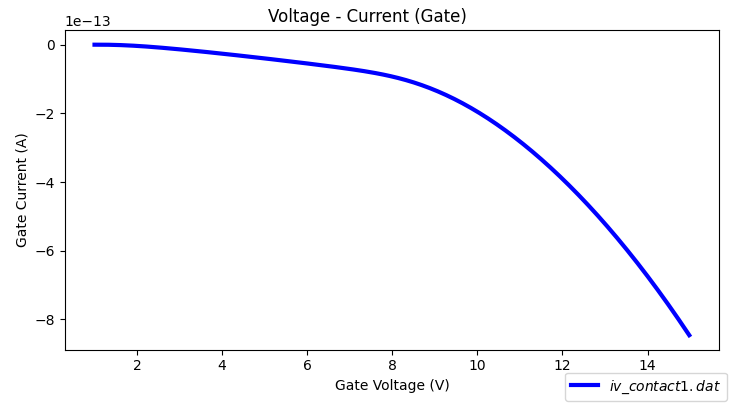
\includegraphics[width=0.5\textwidth,height=0.4\textwidth]{./images/ofet/ofet_8.png}
\\

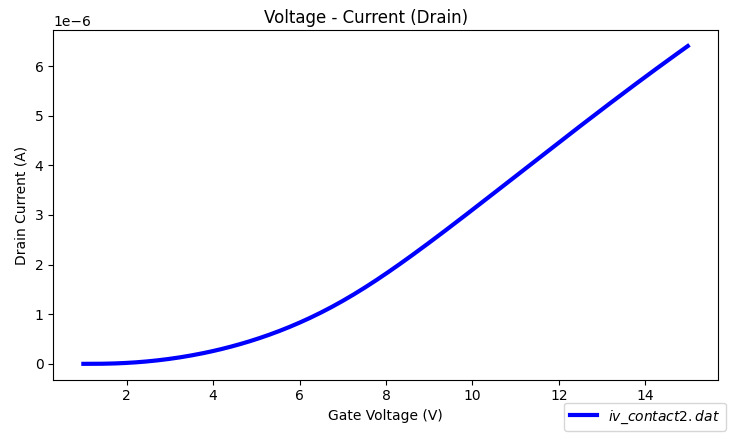
\includegraphics[width=0.5\textwidth,height=0.4\textwidth]{./images/ofet/ofet_9.png}

&
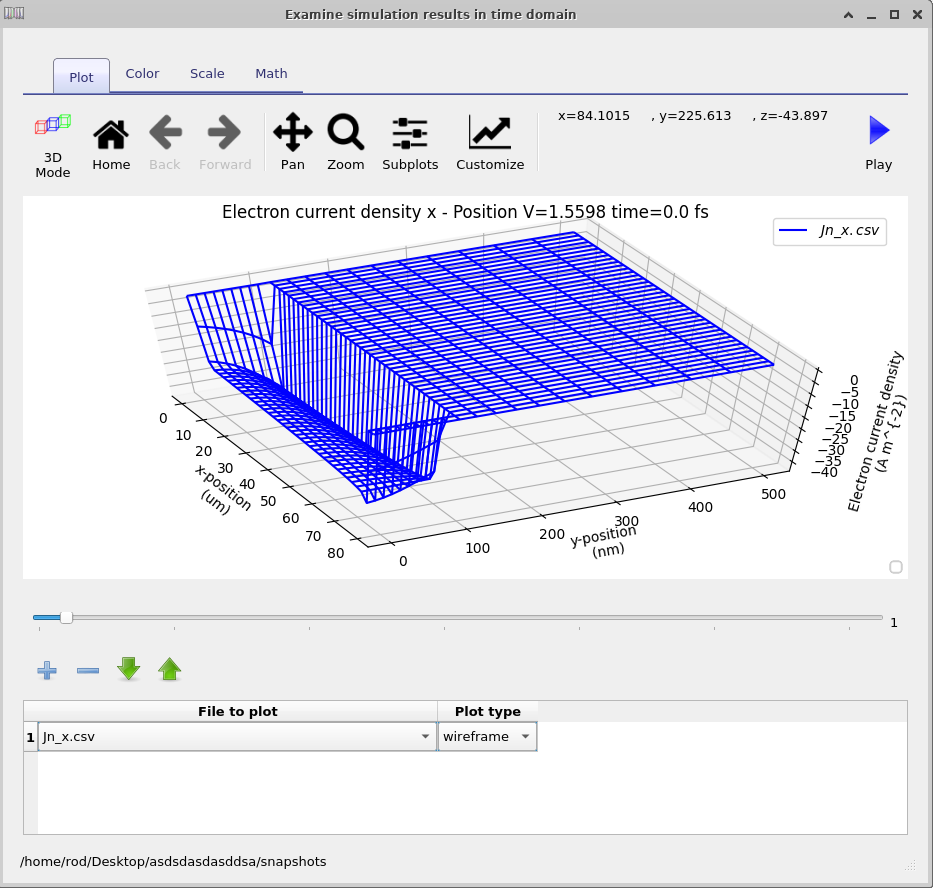
\includegraphics[width=0.5\textwidth,height=0.4\textwidth]{./images/ofet/ofet_10.png}
\\
\end{tabular}
\caption{Results from a 2D OFET simulation the JV curves for each contact are shown along with a view of the the electron current density in the x direction (bottom right).}
\label{tab:ofet_plots}
\end{figure}

\subsection{Meshing in 2D}
\subsubsection{Computational speed, traps and meshing}
You will notice that in this example the SRH trapping/escape equations are solved in the semiconductor layer, you can see this as the SRH trap button is depressed. Trapping is often needed to reproduce experimental results. If you scroll down the parameters list in the Semiconductor layer you will see that it has 8 trap states. However,it is worth taking a moment to consider the computational load of introducing trap states. If our 2D device has $N_x$ mesh points in the x direction and $N_y$ mesh points in the y direction then and we are solving Poisson's equation, the electron drift diffusion equation and the hole drift diffusion equation then we will be solving $3*N_{x}*N_{y}$ equations in total. If we now introduce 8 trap states for electrons and 8 trap states for holes we will then be solving $3*N_{x}*N_{y}+8*2*N_{x}*N_{y}$ equations. So if you want a speedy simulation or are just trying something out it is worth trying to reduce the number of mesh points, and also reduce the number of trap states and/or turn traps off in the first instance.

\subsubsection{Adjusting the mesh}
The electrical mesh editor can be accessed through the electrical ribbon in the main window. The mesh editor is shown in Figure \ref{fig:ofetmeshing}, here the x and y mesh can be adjusted. The number of mesh points directly affects the speed of the computation, as a general rule try to minimize the number of mesh points you use. I would recommend defining one electrical mesh to cover the Semiconductor layer and one to cover the insulator layer.

\begin{figure}[H]
\centering
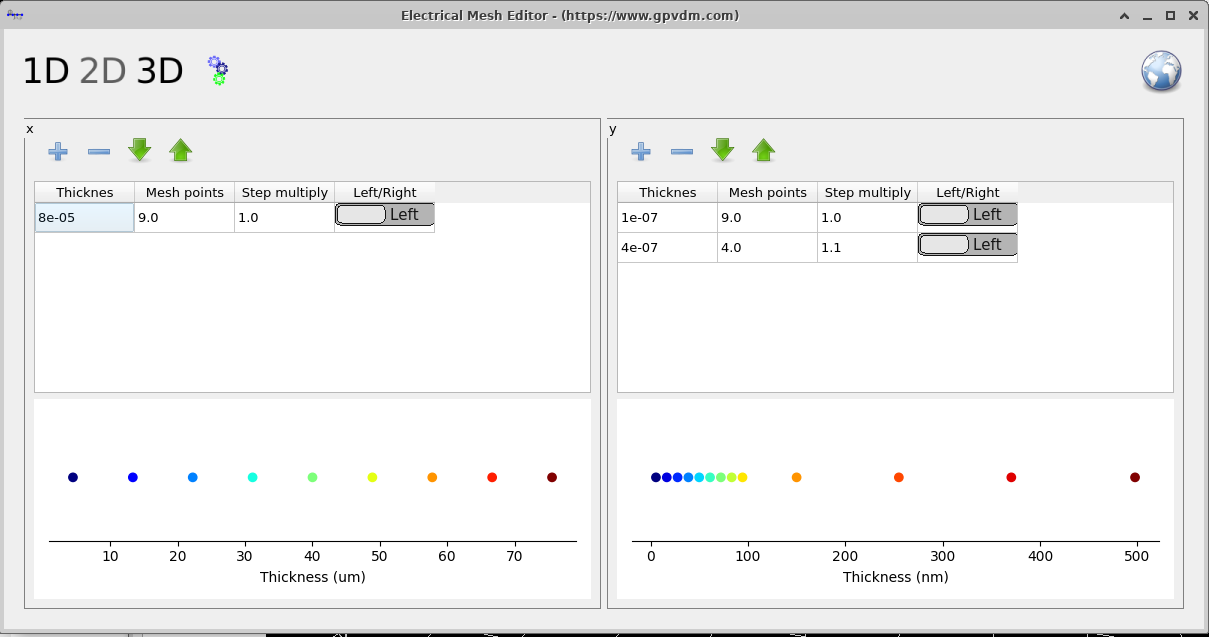
\includegraphics[width=0.7\textwidth]{./images/ofet/ofet_4.png}
\caption{Meshing}
\label{fig:ofetmeshing}
\end{figure}

\subsection{Solving the drift diffusion equations over the entire device}
Sometimes you may want to solve the drift diffusion equations over the entire device this could be because you have a poor insulator on the gate contact, it is very uncommon to want to do this but if you want to follow the steps below. Using doing this is not recommended.
\begin{itemize}
  \item Mobility: Set the mobility of the insulator to a value of  $1x10^{-12}-1x10^{-15} m^{2}/(Vs)$ to limit current flow into the region. However, the value should not be set too low (see section \ref{sec:solverstability}) or the solver may become numerically unstable.
  \item Effective density of states: Keep these the same for both layers, just to keep things simple.
  \item Number of trap states: This must the same in both layers, the density of the states and the Urbach energy can change though.  
  \item Eg and Xi: Although it is tempting to simply enter the experimental values for Xi and Eg for both the insulator and the semiconductor, one has to be careful in doing this as some insulators ($SiO_2$) have very big band gaps which mean the number of carriers get very small and make the simulation unstable (read section \ref{sec:solverstability} for an explanation).  If you want to simulate a jump in the band gap into an insulator, my is to make the jump significantly bigger than $3/2kT=25meV$ which is the average kinetic energy of a charge carrier.  If the gap is between $0.5-1.0 V$ charge carriers will have problems penetrating the barrier and there is no need to simulate bigger steps.
\end{itemize}






